
\section*{练习}
\label{sec:ch02-exercises}

\vkexsync{10}

\begin{exercise}\label{ex:ch02-10}
证明：\cref{fig:not-pseudogradient-flows}中画出其诸\trFlow{}的那些\trVectorField{}都不是\trPseudogradient{}场。
\end{exercise}

\begin{figure}[htbp]
\begin{minipage}[b]{0.48\textwidth}
\centering
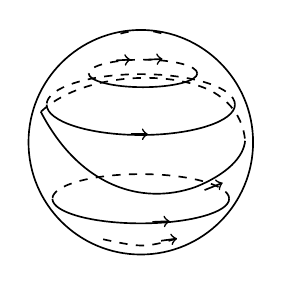
\begin{tikzpicture}[line width=0.6pt,scale=0.92]
  \draw (0,0) circle (1.55);
  \draw (-0.72,0.95) arc[start angle=180,end angle=360,x radius=0.75,y radius=0.19];
  \draw[dashed] (0.78,0.95) arc[start angle=0,end angle=180,x radius=0.75,y radius=0.19];
  \draw[->] (-0.34,1.13) -- (-0.14,1.14);
  \draw[->] (0.10,1.14) -- (0.30,1.15);
  \draw[dashed] (-0.28,1.50) .. controls (0.02,1.57) .. (0.34,1.49);
  \draw (-1.30,0.52) arc[start angle=180,end angle=360,x radius=1.30,y radius=0.42];
  \draw[dashed] (1.30,0.52) arc[start angle=0,end angle=180,x radius=1.30,y radius=0.42];
  \draw[->] (-0.14,0.11) -- (0.10,0.11);
  \draw (-1.38,0.42) .. controls (-0.85,-0.60) and (0.0,-0.88)
        .. (0.75,-0.62) .. controls (1.20,-0.44) and (1.42,-0.20) .. (1.44,0.02);
  \draw[dashed] (-1.38,0.42) .. controls (-0.85,0.92) and (0.3,1.02)
        .. (0.95,0.72) .. controls (1.28,0.55) and (1.42,0.28) .. (1.44,0.02);
  \draw[->] (0.88,-0.66) -- (1.13,-0.56);
  \draw (-1.22,-0.78) arc[start angle=180,end angle=360,x radius=1.22,y radius=0.34];
  \draw[dashed] (1.22,-0.78) arc[start angle=0,end angle=180,x radius=1.22,y radius=0.34];
  \draw[->] (0.16,-1.10) -- (0.40,-1.09);
  \draw[dashed] (-0.52,-1.34) .. controls (0.05,-1.46) .. (0.60,-1.30);
  \draw[->] (0.28,-1.36) -- (0.50,-1.33);
\end{tikzpicture}
\end{minipage}\hfill
\begin{minipage}[b]{0.46\textwidth}
\centering
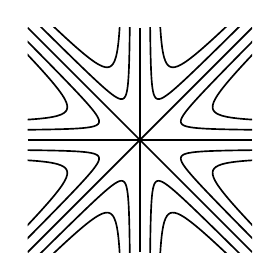
\begin{tikzpicture}[line width=0.6pt,scale=0.92]
  \begin{scope}
    \clip (-1.55,-1.55) rectangle (1.55,1.55);
    \draw (-1.55,0) -- (1.55,0);
    \draw (0,-1.55) -- (0,1.55);
    \draw (-1.55,-1.55) -- (1.55,1.55);
    \draw (-1.55,1.55) -- (1.55,-1.55);
    \foreach \a in {0,45,...,315}
    {
      \begin{scope}[rotate=\a]
        \draw[domain=1.2:43.8,samples=29,smooth]
          plot ({0.09/(sin(\x)*sin(45-\x))*cos(\x)},{0.09/(sin(\x)*sin(45-\x))*sin(\x)});
        \draw[domain=1.2:43.8,samples=29,smooth]
          plot ({0.16/(sin(\x)*sin(45-\x))*cos(\x)},{0.16/(sin(\x)*sin(45-\x))*sin(\x)});
      \end{scope}
    }
  \end{scope}
\end{tikzpicture}
\end{minipage}
\caption{}
\label{fig:not-pseudogradient-flows}
\end{figure}

\begin{exercise}\label{ex:ch02-11}
设 $V$ 是一个维数为 $2$ 的\trManifold，其上赋有一个\trMorseFunction，该函数只有一个\trIndex{}为 $1$ 的\trCriticalPoint。证明：每一个\trAdapted{}于这个函数的\trPseudogradient{}场都满足\trSmaleCondition。
\end{exercise}

\begin{exercise}\label{ex:ch02-12}
我们固定一个整数 $m\ge 2$。求由
\[
f([z_0,z_1])=\frac{|z_0^m+z_1^m|^2}{(|z_0|^2+|z_1|^2)^m}
=\frac{|z^m+1|^2}{(|z|^2+1)^m}
\]
（在\trHomogeneousCoordinates{}下，或者在仿射\trChart{} $z_1\ne 0$ 中）所定义的函数 $f\colon\CP^1(\CC)\to\RR$ 的全部\trCriticalPoint。验证：当 $m=2$ 时，函数 $f$ 不是一个\trMorseFunction。\footnote{它是一个\trMorse{}--\trBott{}函数（参见 [14]）：其诸\trCriticalPoint{}构成诸\trSubmanifold（这里取极大值的那个是 $\CP^1(\RR)$），并且二阶导数沿\trTransverse{}方向\trNondegenerate。（译注：原书此处人名印作“Mores--Bott”；疑应为“Morse--Bott”（显见排印笔误）；此处径改。——译者注）}

我们假定 $m\ge 3$。证明：$f$ 是一个\trMorseFunction，并且它有两个局部极大值，即点 $0$ 与 $\infty$；$m$ 个局部极小值，即 $-1$ 的 $m$ 次根；以及 $m$ 个\trIndex{}为 $1$ 的\trCriticalPoint，即 $1$ 的 $m$ 次根。

\begin{figure}[htbp]
\centering
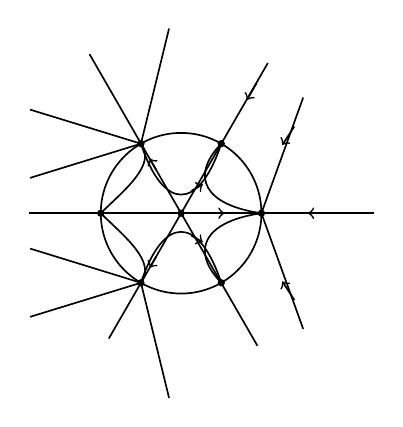
\begin{tikzpicture}[line width=0.6pt,scale=1.02]
  \draw (-1.90,0) -- (2.40,0);
  \draw (-0.90,-1.56) -- (1.08,1.87);
  \draw (0.95,-1.65) -- (-1.14,1.98);
  \draw (1,0) -- (1.52,1.44);
  \draw (1,0) -- (1.52,-1.44);
  \draw (-0.5,0.866) -- (-1.88,0.44);
  \draw (-0.5,0.866) -- (-1.88,1.29);
  \draw (-0.5,0.866) -- (-0.15,2.30);
  \draw (-0.5,-0.866) -- (-1.88,-0.44);
  \draw (-0.5,-0.866) -- (-1.88,-1.29);
  \draw (-0.5,-0.866) -- (-0.15,-2.30);
  \draw (0,0) circle (1);
  \draw (-0.5,0.866) .. controls (-0.30,0.60) and (-0.72,0.28) .. (-1,0);
  \draw (-0.5,-0.866) .. controls (-0.30,-0.60) and (-0.72,-0.28) .. (-1,0);
  \draw (-0.5,0.866) .. controls (-0.22,0.02) and (0.22,0.02) .. (0.5,0.866);
  \draw (-0.5,-0.866) .. controls (-0.22,-0.02) and (0.22,-0.02) .. (0.5,-0.866);
  \draw (1,0) .. controls (0.30,0.10) and (0.10,0.45) .. (0.5,0.866);
  \draw (1,0) .. controls (0.30,-0.10) and (0.10,-0.45) .. (0.5,-0.866);
  \fill (0,0) circle (1.3pt);
  \fill (1,0) circle (1.3pt);
  \fill (-1,0) circle (1.3pt);
  \fill (-0.5,0.866) circle (1.3pt);
  \fill (-0.5,-0.866) circle (1.3pt);
  \fill (0.5,0.866) circle (1.3pt);
  \fill (0.5,-0.866) circle (1.3pt);
  \draw[->] (-0.31,0.54) -- (-0.39,0.68);
  \draw[->] (-0.31,-0.54) -- (-0.39,-0.68);
  \draw[->] (0.32,0) -- (0.54,0);
  \draw[->] (1.82,0) -- (1.58,0);
  \draw[->] (1.41,1.08) -- (1.26,0.85);
  \draw[->] (1.41,-1.08) -- (1.26,-0.85);
  \draw[->] (0.94,1.62) -- (0.82,1.41);
  \draw[->] (0.13,0.28) -- (0.27,0.36);
  \draw[->] (0.13,-0.28) -- (0.27,-0.36);
\end{tikzpicture}
\caption{}
\label{fig:pseudogradient-cubic}
\end{figure}

提示：我们可以利用关于 $z$ 与 $\bar{z}$ 的导数来确定诸\trCriticalPoint，然后在 $0$ 的邻域内对 $f(u)$ 使用关于 $u$ 的二阶\trTaylor{}展开（用以研究 $0$ 与 $\infty$ 处的\trCriticalPoint），或者对 $f\bigl(\zeta(1+u)\bigr)$ 使用类似的展开（用以研究 $\zeta^m=\pm 1$ 的那些 $\zeta$ 处的\trCriticalPoint）。

证明：存在这样的一个\trPseudogradient{}场：它在一张仿射\trChart{}中的图像恰如\cref{fig:pseudogradient-cubic}所示（图中取 $m=3$）。更一般地，可参见文章 [9]，其中一个类似的函数（定义在 $\CP^n(\CC)$ 上）扮演着重要的角色。
\end{exercise}
